\documentclass[12pt,a4paper]{article}
\usepackage{a4wide}
\usepackage[utf8]{inputenc}
\usepackage[greek,english]{babel}
\usepackage{alphabeta}
\usepackage{array}
\usepackage{mathtools}
\usepackage{ragged2e}
\usepackage{graphicx}
\graphicspath{ {./images/} }
\usepackage[most]{tcolorbox}
\newtcolorbox{mybox}[2][]{%
  attach boxed title to top center
               = {yshift=-8pt},
  colback      = white,
  colframe     = black,
  fonttitle    = \bfseries,
  colbacktitle = black,
  title        = #2,#1,
  enhanced,
}
\usepackage[top=60pt,bottom=55pt,left=55pt,right=55pt]{geometry}

\title{Αλγόριθμοι και Πολυπλοκότητα \\* 3η Σειρά Ασκήσεων}
\author{ Καραβαγγέλης Αθανάσιος \\ Α.Μ: 03117022}
\date{12 Ιανουαρίου 2020}

\begin{document}

\maketitle
\newpage

\section*{Άσκηση 1: Ραντεβού μετά το Lockdown } 

\par
Στη συγκεκριμένη άσκηση καλούμαστε ουσιαστικά να βρούμε το μόνοπατι ελάχιστου χρονικά κόστους στο κατευθυνόμενο γράφημα G(V,E) (με n κορυφές και m ακμές) την κορυφή $s \in V$ προς την $t \in V$ (σημείο συνάντησης) ,όπου θεωρούμε ότι το κόστος διάσχισης κάθε ακμής είναι 1 κβάντο χρόνου.\\
\par
Ο αλγόριθμος μου βασίζεται στη δημιουργία ενός νέου μη-κατευθυνόμενου γραφήματος G'(V',E') ,όπου V' = 2V και $ Ε' > Ε $ το οποίο δημιουργείται με τους εξής κανόνες:
\begin{itemize}
    \item Αρχικά για κάθε κόμβο, έστω a, του γραφήματος G θα ορίσουμε στο G' δύο κόμβους , έναν $a_{odd}$ και έναν $a_{even}$ που θα αφορούν περιττές και άρτιες χρονικές στιγμές αντίστοιχα. Γι'αυτό και V' = 2V.
    \item Έπειτα για κάθε ακμή $e \in E$ όπου e = ($k,l$) ,που δηλαδή αναπαριστά την ακμή από τον κόμβο k στον l, θα ορίσουμε μία νέα ακμή ($k_{odd}$,$l_{even}$) με βάρος 1 στον G' ,δεδομένου ότι ο G που μας δίνεται αντιστοιχεί στις περιττές χρονικές στιγμές με βάση την εκφώνηση. Έτσι διασφαλίζεται ότι κάθε χρονική στιγμή ,είτε αυτή είναι odd είτε even, έχουμε συγκεκριμένες επιλογές όσον αφορά την διαδρομή μας πάνω στο γράφο , οι οποίες θα είναι οι αντίστοιχες ακμές στον G'.
    \item Τέλος, θα ορίσουμε n ακμές στο G' με βάρος 1, για κάθε ζεύγος odd και even που αναφέρονται στον ίδιο κόμβο του G, οι οποίες ουσιαστικά θα αναπαριστούν την αναμονή για 1 κβάντο χρόνου στον ίδιο κόμβο.\\\\
\end{itemize} 

Ένα παράδειγμα γραφημάτων G και G' φαίνεται παρακάτω για n = 5 και m = 7 . \\

\begin{figure}[h]
    \begin{tabular}{ll}
    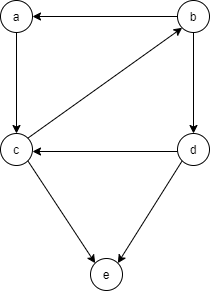
\includegraphics[scale=0.7]{images/dag_for_1.png}
    &
    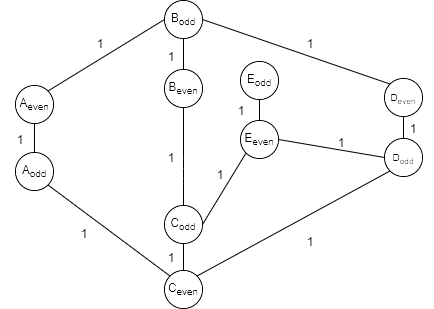
\includegraphics[scale=0.8]{images/nondag_for_1 (1).png}
    \end{tabular}
    \caption{Αριστερά: Παράδειγμα γραφήματος G . Δεξιά: Παράδειγμα γραφήματος G'.}
\end{figure}



Έτσι , τελικά θα έχουμε τον νέο μη-κατευθυνόμενο γράφο G' στον οποίο θα πρέπει να βρούμε το συντομότερο μονοπάτι από τους κόμβους $s_{odd}$ και $s_{even}$ σε έναν εκ των $t_{odd}$ ή $t_{even}$.


\par 
Για την εύρεση του συντομότερου αυτού μονοπατιού θα πρέπει να χρησιμοποιήσουμε τον αλγόριθμο BFS (Breadth-First Search) . Αυτός θα εφαρμοστεί 2 φορές , τη μία έχοντας ρίζα τον $s_{odd}$ και την αλλή τον $s_{even}$ ,εξερευνώντας όλους τους γειτονικούς κόμβους της ρίζας προτού μεταβεί στους γείτονες του επόμενου επιπέδου. 

\par
Αν ο αλγόριθμος μας βρει ως απάντηση έναν χρόνο έστω $t_{min}$ που απαιτείται για να φτάσει κανείς από τον κόμβο s στον t ,τότε πρέπει να επιστραφεί ως αποτέλεσμα η χρονική στιγμή \\ 
Τ - $t_{min}$ ως η τελευταία χρονικά έγκυρη στιγμή που μπορεί να ξεκινήσει κάποιος από τον s ώστε 
να φτάσει έγκαιρα στον t.
\begin{center}
    \textbf{Ψευδοκώδικας}
\end{center}

\begin{mybox}[colback=white]{My Algorithm}
\begin{tabbing}
1 procedure \= MyAlgorithm( G(V,E) , G'(V',E') , T) is \\
2 \>for \= each vertex $v \in V$ do \\
3 \>\> ADDVERTEX($v_{odd}$,G')                      //procedure to add vertexes to a graph \\
4 \>\> ADDVERTEX($v_{even}$,G')\\
5 \>for \= each edge $(k,l) \in E$ do\\
6 \>\> ADDEDGE($k_{odd}$,$l_{even}$,G')             //procedure to add edges to a graph \\
7 \>for \= each vertex $v \in V$ do \\
8 \>\> ADDEDGE($v_{odd}$,$v_{even}$,G') \\
9 \>solution1 $\leftarrow$ BFS(G',$s_{odd}$) \\
10 \>solution2 $\leftarrow$ BFS(G',$s_{even}$) \\
11\>return Τ - min(solution1,solution2)
\end{tabbing}
\end{mybox}
O κώδικας του BFS για ένα γράφο G εκκινώντας από τον κόμβο root(διαφάνειες μαθήματος, Αναζήτηση Κατά Πλάτος) έχοντας :\\Έναν πίνακα κατάστασης m[u] = {A,Y,E} καθώς και \\Έναν πίνακα γονέων p[u] = πατέρας κόμβου u στο BFS δάσος  \\
\begin{mybox}{BFS}
\begin{tabbing}
 1 procedure \=BFS(G(V,Ε), root) is \\
 2      \>addToQueue(root)\\
 3      \>m[s]$\leftarrow$Y\\
 4      \>p[s]$\leftarrow$null\\
 5      \>for \=all $u \in V$ \textbackslash \{s\} do \\
 6           \>\>m[u] $\leftarrow$ A\\
 7           \>\>p[u]$\leftarrow$ null \\
 8      \>while \=  not emptyQueue() do\\
 9          \>\>u$\leftarrow$ extractFromQueue() \\
 10         \>\>m[u] $\leftarrow$ E\\
 11         \>\>for \=all $u \in L[u]$ do\\
12         \>\>\>if \=m[u] = A then\\
13                  \>\>\>\>addToQueue(u)\\
14                   \>\>\>\>m[u]$\leftarrow$Y\\
15                   \>\>\>\>p[u]$\leftarrow$u
\end{tabbing}
\end{mybox}
\newpage
\begin{center}
    \textbf{Πολυπλοκότητα}
\end{center}

Όσον αφορά την πολυπλοκότητα του αλγορίθμου που πρότεινα αυτή είναι ως εξής. Αρχικά , για την δημιουργία του νέου γράφου η πολυπλοκότητα είναι O(2V+E) δηλαδή O(V+E). Έπειτα , για τις 2 BFS η πολυπλοκότητα είναι Ο(2(V'+E')) δηλαδή O(V+E). \textbf{Άρα τελικά η χρονική πολυπλοκότητα μας έιναι Ο(V+E).} \\
\par H χωρική πολυπλοκότητα του αλγοριθμού μας είναι O(|V'|) για τον αλγόριθμο BFS και για την αποθήκευση των 2 γράφων είναι O($V^2$ + ${V'}^2$).\textbf{ Άρα τελικά η χωρική πολυπλοκότητα μας είναι O($V^2$ + ${V'}^2$).}\\\\

\section*{Άσκηση 2: Προγραμματίζοντας την αντίδραση }

\par 
Στο συγκεκριμένο πρόβλημα καλούμαστε να προγραμματίσουμε την κίνηση k σωματιδιών $q_1,q_2,...,q_k$
τα οποία βρίσκονται σε k άγνωστες αρχικές θέσεις πάνω σε ένα μη-κατευθυνόμενο γράφημα G(V,E). Αν ένα σωματίδιο βρίσκεται την ημέρα t σε έναν κόμβο ,τότε μπορεί να μετακινηθεί μόνο σε γειτονικούς κόμβους ή να παραμείνει στην ίδια θέση την επόμενη μέρα t+1. Δε μπορούμε ωστόσο να ελέγξουμε τι από τα δύο θα κάνει . Ακόμη, όλα τα σωματίδια μετακινούνται ταυτόχρονα τα μεσάνυχτα κάθε ημέρας γεγονός που μας βοηθάει για τον προγραμματισμό της κίνησης τους . \\ 

\par 
O αλγόριθμος που θα ακολουθήσουμε για την επίλυση του προβλήματος αυτού έχει ως εξής : 
\begin{itemize}
    \item Αρχικά ,θα ξεκινήσουμε εκτελώντας πριν την ημέρα 1 σειριακά k φόρες BFS (Breadth-First Searches) κάθε φορά εκκινώντας από την αρχική θέση ενός διαφορετικού από τα k σωματίδια,έχοντας δηλαδή k διαφορετικούς $root_j$,όπου j =1,2,...,k . Θα αποθηκεύουμε τον αριθμό βημάτων που απαιτούνται για την έλευση σε κάθε κόμβο από κάθε ένα από τους k roots, καθώς και τον κόμβο "γονέα" του κάθε κόμβου. 
    \item Ο πρώτος κόμβος τον οποίο θα επισκεφθούν και τα k σωματίδια (μέσω των BFS) θα είναι ο κόμβος αυτός που θα πρέπει να συναντηθούν τα σωματίδια ώστε να συμβεί η αντίδραση το συντομότερο δυνατό. Έτσι από αυτόν τον κόμβο ξεκινάμε ένα λεγόμενο "backtrack" μέχρι τον αντίστοιχο κόμβο $root_j$ ,όπου j = 1,2,...,k. Θα προγραμματίσουμε λοιπόν σύμφωνα με αυτά τα k μονοπάτια την κίνηση των k σωματιδίων.
    \item Την επόμενη ημέρα , αν κανένα από τα k σωματίδια δεν έχει κινηθεί ή αν έχουν κινηθεί όλα τα σωματίδια δε χρειάζεται να εκτελέσουμε ξανά κάποια αναζήτηση. Ωστόσο , αν έχουν κινηθεί μόνο κάποια από τα k σωματίδια ,με τα υπόλοιπα να παραμένουν στις θέσεις τους , θα πρέπει να εκτελέσουμε ξανά k φορές τον αλγόριθμο BFS , ακριβώς όπως παραπάνω , καθώς το πρόβλημα μας έχει επαναπροσδιοριστεί . Θα βρούμε έναν νέο κόμβο συνάντησης με βάση τον οποίο θα επανάπρογραμματίσουμε τα σωματίδια.
    \item Επαναλαμβάνουμε τα παραπάνω μέχρι όλα τα σωματίδια να βρεθούν στον ίδιο κόμβο και να γίνει η αντίδραση,την t-ιοστή ημέρα.\\
\end{itemize}
\newpage 
\par Η \textbf{ορθότητα} του αλγορίθμου έγγυται στην ορθότητα του αλγορίθμου BFS  ο οποίος διασχίζει κατα πλάτος το γράφημα G και στην ορθή επιλογή του "βέλτιστου" κόμβου συνάντησης που προκύπτει από αναζήτηση σε κάθε χρονική στιγμή μέχρι να βρεθεί κόμβος που τον έχουν επισκεφθεί και οι k BFS αλγόριθμοι. Ο κόμβος αυτός θα είναι ο "βέλτιστος" αφού σε προηγούμενες στιγμές δε θα υπάρχει κόμβος που να έχουν συναντηθεί και τα k σωματίδια.

\begin{center}
    \textbf{Πολυπλοκότητα}
\end{center}

Η πολυπλοκότητα για τον αλγόριθμο BFS είναι O(V + E) και στη χειρότερη περίπτωση τον εκτελούμε και στις t ημέρες μέχρι τη συνάντηση των σωματιδίων από k φορές την ημέρα ,δηλαδή συνολικά \textbf{ O(tk(V + E)). }
\par Η χωρική πολυπλοκότητα για τον αλγόριθμο είναι O(kV) για τους πίνακες γονέων , Ο(kV) για τους πίνακες για τον αριθμό βημάτων που απαιτήθηκαν μέχρι κάθε κόμβο και O($V^2$) για το γράφημα, άρα συνολικά {O($V^2$)}.\\\\

\section*{Άσκηση 3: Ένας Παράξενος Περίπατος }

Το συγκεκριμένο πρόβλημα μοιάζει με το πρόβλημα του συντομότερου μονοπατιού με μία διαφοροποίηση. Το συντομότερο μονοπάτι στην άσκηση δε συνίσταται στο ελάχιστο άθροισμα από τα βάρη των κορυφών του αλλά στον ελάχιστο μέγιστο κοινό διαιρέτη κορυφών του μονοπατιού. \\
\par
Για την υλοποίηση του αλγορίθμου θα θεωρήσουμε ότι για το ελάχιστο κόστος του περιπάτου μας συμπεριλαμβάνουμε και κύκλους στους περιπάτους.\\
\par 
Ο αλγόριθμος που θα ακολουθήσουμε για το πρόβλημα είναι ο Floyd Warshall. Ο συγκεκριμένος αλγόριθμος υπολογίζει κανονικά τα συντομότερα μονοπάτια από οποιονδήποτε κόμβο σε οποιονδήποτε άλλο σε ένα γράφημα G. Ωστόσο , με κάποιες σημαντικές διαφοροποιήσεις θα μας βοηθήσει να βρούμε τα ελάχιστα κόστη περιπάτων από έναν κόμβο σε κάποιον άλλο.\\
\par Αρχικά θα χρησιμοποιήσουμε έναν πίνακα (VxV) στον οποίο στη θέση (i,j) θα κρατάμε μία λίστα με τους κόμβους που συνιστούν τον περίπατο με το ελάχιστο κόστος από τον κόμβο $u_i$ στον κόμβο $u_j$. Έπειτα θα τροποποιήσουμε τον αλγόριθμο του Floyd Warshall ως εξής:
\begin{mybox}{MyFloydWarshall}
let walks be a (VxV) array of lists initialized to [$\infty$] for a walk where walk[i][j] = list of nodes in walk from node i to node j //if a walk is not possible walk[i][j] = [$\infty$] 
\begin{tabbing}
 1 procedure \= MyFloydWarshall(G(V,E,c)) is \\
 2 \>for \= each edge ($u_i,u_j$) $\in E$ do \\
 3\>\>walk[i][j] $\leftarrow$ ($u_i,u_j$) \\
 4\>for each vertex $u_i \in V$ do\\
 5\>\>walk[i][i]$\leftarrow$[$u_i$]\\
 6\>for \=k from 1 to $\mid V \mid $do \\
 7\>\>for \=i from 1 to $\mid V \mid$ do \\
 8\>\>\>for \=j from 1 to $\mid V \mid$ do \\
 9\>\>\>\>if \=gcd(walk[i][j]) $>$ gcd(MergeLists(walk[i][k],walk[k][j])) then\\
 10\>\>\>\>\>walk[i][j]$\leftarrow$MergeLists(walk[i][k],walk[k][j])
\end{tabbing}
\end{mybox}

\par Στον παραπάνω ψευδοκώδικα του αλγορίθμου που προτείνω παρατηρούμε ότι αντί στην if να γίνεται σύγκριση μεταξυ της ηδη υπάρχουσας τιμής στον πίνακα και ενός αθροίσματος ,τώρα γίνεται σύγκριση των μέγιστων κοινών διαιρετών 2 λιστών. Ωστόσο, "τρέχοντας" τον αλγόριθμο μία φορα θα παρατηρήσουμε ότι δε συμπεριλαμβάνει κύκλους ,καθώς ο αλγόριθμος έχει δημιουργηθεί για να βρίσκει συντομότερα μονοπάτια ,τα οποία δε περιλαμβάνουν κύκλους. Ωστόσο , τρέχοντας μία δεύτερη συνεχόμενη φορά τον αλγόριθμο για το γράφημα ,θα συμπεριληφθούν και κύκλοι καθώς στις θέσεις του πίνακα θα έχουμε πλέον διαθέσιμα όλα τα ελάχιστου κόστους μονοπάτια , των οποίων ο συνδυασμός εξάγει και κύκλους .
\par Επομένως , θα εφαρμόσουμε 2 συνεχόμενες φορές τον αλγόριθμο MyFloydWarshall και η απάντηση στην ερώτηση ποιος είναι ο περίπατος ελαχίστου κόστους από τον κόμβο $u_i$ στον $u_j$ θα είναι gcd(walk[i][j]).
\begin{center}
    \textbf{Πολυπλοκότητα}
\end{center}

\par Η χρονική πολυπλοκότητα του αλγορίθμου μας θα είναι Ο(2$\mid V\mid ^3$) ,δηλαδή Ο($\mid V\mid ^3$),εφόσον εκτελούμε 2 φορές τον MyFloydWarshall που περιέχει 3 for loops από 1 έως $\mid V\mid$. Να αναφέρουμε πως ο υπολογισμός του gcd είναι γραμμικός και δεν επηρεάζει την πολυπλοκότητα του αλγορίθμου μας .
\par Η χωρική πολυπλοκότητα του αλγορίθμου μας θα είναι O($V^2$) αφού χρησιμοποιούμε πίνακα (VxV) για την αποθήκευση των λιστών των περιπάτων.

\section*{Άσκηση 4: Ελάχιστο Συνδετικό Δέντρο με Περιορισμούς }
\subsection*{α.}
Για το πρώτο ερώτημα θα χρησιμοποιήσουμε ένα αντιπαράδειγμα που μας δείχνει το επιθυμητό συμπέρασμα. Έστω ο παρακάτω γράφος:
\begin{figure}[h]
    \centering
    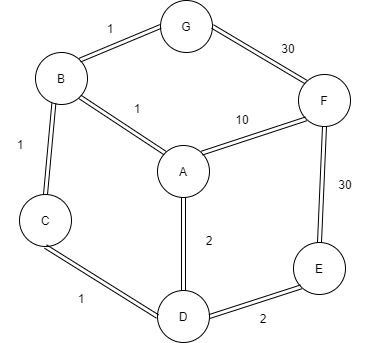
\includegraphics[scale = 0.6]{images/ask4(1).png}
    \caption{Παράδειγμα ενός γραφήματος G.}
    \label{fig2}
\end{figure}

\par Έστω ότι στο συγκεκριμένο γράφημα θέλουμε να έχουμε 2 ακμές στον κόμβο A. Τότε το ελάχιστο συνδετικό δέντρο που θα προέκυπτε από το greedy κριτήριο θα έιχε συμπεριλάβει τις ακμές A-B και A-D καθώς αυτές με κόστη 1 και 2 είναι οι μικρότερες. Όμως το συνδετικό δέντρο που θα προέκυπτε θα είχε συνολικό κόστος 37,αφού θα έπρεπε να συμπεριλάβουμε και την E-F ή την G-F βάρους 30. 
\par Στο παρακάτω σχήμα , φαίνεται το σωστό ελάχιστο συνδετικό δέντρο όπιυ δε συμπεριλαμβάνεται η A-D αλλά η A-F καθώς με αυτό τον τρόπο το συνολικό κόστος είναι 16 , πολύ λιγότερο από 37 .
\begin{figure}[h]
    \centering
    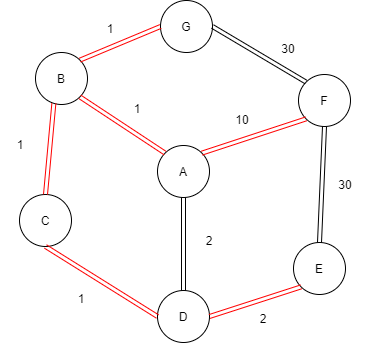
\includegraphics[scale = 0.6]{images/ask4.png}
    \caption{Ελάχιστο Συνδετικό Δέντρο γραφήματος G.}
    \label{fig2}
\end{figure}

\par Συνεπώς, βλέπουμε πως η μη επιλογή των ακμών με το greedy κριτήριο μας οδηγεί σε ελάχιστο συνδετικό δέντρο , άρα η άπληστη στρατηγική δε μας οδηγεί πάντα σε ελάχιστο συνδετικό δέντρο. 

\subsection*{β.}

\par Χρειάζομαστε έναν αλγόριθμο ο οποίος θα βρίσκει ένα ελάχισο συνδετικό δέντρο Τ*(s,k) στο οποίο η κορυφή s να έχει βαθμό ίσο με k.\\
\par Αρχικά, αν ο κόμβος s έχει στο γράφημα k ακμές που άπτονται σε αυτόν τότε παίρνουμε όλες τις ακμές του και έπειτα με τη βοήθεια ενός αλγορίθμου εύρεσης ελάχιστου συνδετικού δέντρου βρίσκουμε τις υπόλοιπες ακμές του δέντρου θεωρώντας ότι ο s μαζί με τις ακμές του  και τους κόμβους στα άλλα άκρα αυτών αποτελούν μία συνιστώσα. Έτσι , εν τέλει θα πάρουμε ένα ελάχιστο συνδετικό δέντρο με τον κόμβο s να έχει k ακμές σε αυτό.\\

\par Στην περίπτωση που ο κόμβος s δεν έχει k ακμές που άπτονται σε αυτόν, θα λειτουργήσουμε ως εξής.
\begin{itemize}
    \item Αρχικά αφαιρούμε από το γράφημα G τον κόμβο s καθώς και τις ακμές του.
    \item Έπειτα για κάθε μία από τις συνιστώσες που θα προκύψουν ,θα υπολογίσουμε το ελάχιστο συνδετικό δέντρο τους με τη βοήθεια κάποιου αλγορίθμου όπως ο Boruvka. 
    \item Έπειτα επαναφέρουμε τον κόμβο s και κρατάμε μόνο τις ελάχιστες ακμές του κόμβου που τον συνδέουν με κάθεμια από τις συνιστώσες που προέκυψαν.
    \item Αν οι ακμές που έχουμε στον κόμβο s τώρα είναι ίσες με k ,τότε η λύση τελειώνει εδώ. Αν όμως ο αριθμός των ακμών είναι μικρότερος του k θα ακολουθήσουμε τα εξής.
    \item Για κάθε μία από τις ακμές $e_i$ του s που δεν επιλέξαμε ως τις ελάχιστες που τον συνδέουν με τις διάφορες συνιστώσες ,έστω i ο αριθμός τους, θα κάνουμε τα εξής. Αυτές θα συνδέουν τον s με κάποιο γείτονα του στο G έστω $u_i$. Θα υπολογίσουμε τη μέγιστη σε βάρος ακμή, μέσω BFS, που υπάρχει στο μονοπάτι s - $u_i$ , έστω $max_i$. Θα ορίσουμε τέλος ένα κόστος $c_i$ = w($max_i$) - w($e_i$) που θα μας δείχνει πόσο θα κερδίσουμε ή θα χάσουμε αντίστοιχα ,αν προσθέσουμε την ακμή $e_i$ στο δέντρο αφαιρώντας παράλληλα την $max_i$.\\
    Θα εισάγουμε τις τετράδες ($e_i,u_i,max_i,c_i$) σε μία ουρά ταξινομημένες με βάση το $c_i$.Όσο δεν έχουμε k ακμές στον s θα εξάγουμε μια τετράδα από την ουρά και θα αντικαθιστούμε στο δέντρο την $max_i$ με την $e_i$. Ο αλγόριθμος θα σταματήσει όταν φτάσουμε να έχουμε k ακμές στον s.
    \item Ο αλγόριθμος αυτός μας δίνει το σωστό αποτέλεσμα αφού κάθε φορά προσθέτουμε στο δέντρο την ακμή που βελτιώνει ή χειροτερεύει με τον βέλτιστο τρόπο το συνολικό κόστος του δέντρου μας . Έτσι θα καταλήξουμε στο ελάχιστο συνδετικό δέντρο με τον ζητούμενο περιορισμό 
\end{itemize}

\begin{center}
    \textbf{Πολυπλοκότητα}
\end{center}

Η χρονική πολυπλοκότητα του αλγορίθμου μας είναι Ο($\mid V \mid + \mid E\mid$) για τον υπολογισμό των $max_i$ ακμών μέσω BFS . Ο αλγόριθμος Boruvka έχει πολυπλοκότητα O($\mid E \mid log\mid V\mid$) ,άρα συνολικά έχουμε πολυπλοκότητα O($\mid E \mid log\mid V\mid$).
\par Η χωρική πολυπλοκότητα είναι O($\mid V \mid$) για την ουρά προτεραιότητας και Ο($\mid V \mid^2$) για την αποθήκευση του γράφου. Άρα συνολικά Ο($\mid V \mid^2$) .


\section*{Άσκηση 5: }
\subsection*{α.}

\par Αρχικά , ο αλγόριθμος Boruvka εκκινεί θεωρώντας κάθε κόμβο μόνο του ως μία ξεχωριστή συνιστώσα .Για κάθε μία από τις συνιστώσες επιλέγουμε την ελάχιστη ακμή που προσπίπτει σε αυτές και την τοποθετούμε στο δάσος που έχουμε . Έπειτα ενημερώνουμε τον αριθμό των συνιστωσών που έχουμε ,και επαναλαμβάνουμε για τις νέες συνιστώσες μέχρι να έχουμε μόνο μία συνιστώσα , η οποία θα είναι και το Ελάχιστο Συνδετικό Δέντρο .

\subsubsection*{i)}

\par \textbf{1η Περίπτωση} : Έστω ότι μετά την εκτέλεση του αλγορίθμου Boruvka δε λαμβάνω συνδετικό δέντρο. Θα πρέπει λοιπόν να έχουμε καταλήξει σε δέντρα $Τ_1$ και $T_2$ που να μην μπορώ να ενώσω.Αυτό όμως είναι άτοπο αφού το γράφημα είναι συνεκτικό και άρα υπάρχει για κάθε κόμβο του $Τ_1$ μονοπάτι που να τον ενώνει με το $Τ_2$.\\\\
\textbf{2η Περίπτωση} : Η ακμή(u,v) που ελέγχουμε και είναι η ελάχιστη στο $Τ_1$  δημιουργεί κύκλο στο $Τ_2$. Αυτό σημαίνει ότι τα 2 δέντρα θα είναι υπογράφοι κάποιου άλλου δέντρου που έχει υπολογιστεί . Άρα,λοιπόν θα έχουν υπολογιστεί ακμές που οδηγούν από το u στο v χωρίς την ακμή (u,v) . Τότε αν έχω ένα μονοπάτι $T_1,e_1,Τ_α,e_2,....,e_i,T_2$ σημαίνει ότι η ακμή (u,v) είναι διαφορετική της $e_1$ κι εφόσον είναι η ελάχιστη που προσπίπτει στο $Τ_1$ θα ισχύει c((u,v)) < c($e_1$). Ακόμη, για να επιλεγεί η $e_1$ σημαίνει ότι είναι η μικρότερη σε βάρος ακμή που προσπίπτει στο $Τ_α$ και ούτω καθεξής. Οπότε ,τελικά θα ισχύει $c(e)<c(e_1)<c(e_2)<...<c(e_i)$. Αυτό όμως συνεπάγεται ότι η $e_i$ πρέπει να είναι η ακμή που προσπίπτει στο $Τ_2$ και έχει το μικρότερο βάρος ,που όμως λόγω υπόθεσης είναι άτοπο άφου αυτή είναι η e. \\\\
Επομένως σε κάθε μία από τις 2 περιπτώσεις ο αλγόριθμος του Boruvka καταλήγει σε συνδετικό δέντρο.

\subsubsection*{ii)}

Έστω Τ το δέντρο που προκύπτει από τον αλγόριθμο του Boruvka και Τ' το ελάχιστο συνδετικό δέντρο. Έστω ότι $Τ \ne T'$ και e η κορυφή που ανήκει στο Τ και όχι στο Τ'. Ορίζω ως p το μονοπάτι που ενωνει τους κόμβους που ενώνει η e στο Τ. Εφόσον η ακμή e έχει επιλεγεί από τον αλγόριθμο του Boruvka , αυτό συνεπάγεται πως τουλάχιστον μία από τις ακμές ,έστω e',που ανήκει στο p δεν έχει επιλεγεί. Ωστόσο , σύμφωνα με τον αλγόριθμο θα έχουμε ότι w(e') > w(e). Όμως έχουμε πει ότι το Τ' είναι το ελάχιστο συνδετικό δέντρο ,το οποίο όμως είναι άτοπο αφού δεν περιέχει την ακμή e η οποία ελαχιστοποιεί τα βάρη. Άρα ο αλγόριθμος του Boruvka οδηγεί πάντα σε Ελάχιστο Συνδετικό Δέντρο.

\subsection*{b.}
Μία υλοποίηση του αλγορίθμου Boruvka είναι η παρακάτω . Αυτή χρησιμοποιεί μία συνάρτηση CountandGiveLabels η οποία μετράει τις συνιστώσες και τις ονομάζει με διαφορετικά ονόματα. Επίσης χρησιμοποιεί μία συνάρτηση AddAppropriateEdges η οποία ουσιαστικά κάνει αυτό που λεει το όνομα της , δηλαδή προσθέτει σε κάθε συνιστώσα τις ελάχιστες ακμές που προσπίπτουν σε αυτές. Η δεύτερη χρησιμοποιεί έναν πίνακα S στον οποίο αποθηκεύουμε στη θέση S[i] την ελάχιστη ακμή που προσπίπτει στην i-οστή συνιστώσα. Για τον υπολογισμό του πίνακα αυτού ,ψάχνουμε όλες τις ακμές που ανήκουν στο Ε .Αν τα 2 άκρα της ακμής βρίσκονται στην ίδια συνιστώσα την προσπερνάμε , αλλιώς συγκρίνουμε το βάρος της ακμής με την ελάχιστη ακμή σε κάθε μία από τις συνιστώσες των κορυφών που προσπίπτει. Αν είναι μικρότερο αυτό το βάρος τότε ενημερώνουμε καταλλήλως τον πίνακα.

\begin{mybox}{Boruvka}
    \begin{tabbing}
1    proc\=edure Boruvka(G(V,E)) is\\
2        \>F = (V, $\emptyset$)\\
3        \>count $\leftarrow$ CountandGiveLabels(F) \\
4        \>while \= $count > 1$ \\
5        \>\>AddAppropriateEdges(E,F,count)\\
6        \>\>count$\leftarrow$CountandGiveLabels(F)\\
7        \>return F
    \end{tabbing}
\end{mybox}
    
\begin{mybox}{Add Appropriate Edges}
    \begin{tabbing}
1    proc\=edure AddAppropriateEdges(E,F,count) is \\
2    \>for \= i $\leftarrow$ 1 to count \\
3    \>\>S[i]$\leftarrow$NULL //W(NULL) = $\infty$ \\
4    \>for \=each edge $uv \in E$\\
5    \>\>if \=label(u) $\ne$ label(v)\\
6    \>\>\>if \=w(uv) $<$ w(S[label(u)])\\
7    \>\>\>\>S[label(u)] $\leftarrow$uv \\
8    \>\>\>if \=w(uv) $<$ w(S[label(v)])\\
9    \>\>\>\>S[label(v)] $\leftarrow$uv \\
10    \>for \=i $\leftarrow $1 to count \\
11    \>\> if \=S[i] $\ne$ NULL\\
12    \>\>\>add S[i] to F
    \end{tabbing}
        
\end{mybox}

Η πολυπλοκότητα του αλγορίθμου είναι Ο(mlogn) αφού η while loop μειώνει τις συνιστώσες κάθε φορά τουλάχιστον στις μισές δηλαδή τρέχει στη χειρότερη περίπτωση log$\mid V\mid$ = logn φορές, ενώ η 2η for loop τρέχει στη χειρότερη περίπτωση $\mid E \mid$ = m φορές . Άρα η πολυπλοκότητα είναι O(mlogn).
  
\subsection*{γ.}
Θα ακολουθήσουμε τα εξής βήματα :
\begin{itemize}
\item Αρχικά θα περιορίσω τον αλγόριθμο του Boruvka σε loglogn επαναλήψεις έτσι αντί να πάρω μόνο ένα δέντρο στο τέλος θα πάρω n/logn δέντρα.
\item Στη συνέχεια στο νέο γράφημα G' που προέκυψε χρησιμοποιώ τον αλγόριθμο του Prim με σωρούς Fibonacci και έτσι σε χρόνο Ο(VlogV+E),V = n/logn και E=m ,παίρνω ένα δέντρο.
\item Απλοποιώ το δέντρο αυτό με βάση τα δέντρα που έχει βρει ο Boruvka στην αρχη ,και έτσι θα έχω το ελάχιστο συνδετικό δέντρο με πολυπλοκότητα Ο(mloglogn).
\end{itemize}

\subsection*{δ.}
Ξεκινάω από ένα γράφημα G που ανηκει σε μία βολική κλάση γραφημάτων.Για κάθε έναν από τους κόμβους επιλέγω την ελαφρύτερη ακμή που προσπίπτει σε αυτόν. \\
Έπειτα δημιουργώ,υπερκόμβους ενώνοντας τα στοιχεία που είχαν τις ελαφρύτερες ακμές .\\
Πραγματοποιώ τα παραπάνω μέχρι να έχουμε σύνολο δέντρων ίσο με 1.\\
Στον αλγόριθμο του Boruvka σε κάθε στάδιο έχω τουλάχιστον υποδιπλασιασμό των συνιστωσών ,άρα θα έχω πολυπλοκότητα ίση με Ο($\mid V \mid+\mid V/2\mid+\mid V/4\mid+...+1$ = O($\mid V\mid$).
    
    
    
\section*{Άσκηση 6: Το Σύνολο των Συνδετικών Δέντρων}

\subsection*{α.}
Αρχικά , αν αφαιρέσουμε μία ακμή e από το $Τ_1$ ,τότε το $Τ_1$ δε θα είναι πια δέντρο αλλά δάσος. Αυτό μπορεί να αποδειχθεί από τον ορισμό του Συνδετικού Δέντρου όπου αναφέρεται ότι είναι συνδετικό με τον ελάχιστο αριθμό ακμών οπότε αν αφαιρέσουμε μία ακμή θα έχουμε ένα δάσος.\\\\
Τώρα, έχοντας μία τομή στο πρώτο γράφο ,γνωρίζουμε πως κατα την κασκευή του $Τ_2$ χρησιμοποιήσαμε μία ακμή e' για να "γεφυρώσουμε" την ίδια τομή . Επομένως το τελικό δέντρο\\ $(T_1 $\textbackslash \{e\}) $\bigcup$ \{e'\} θα είναι συνδετικό δέντρο.\\\\
Ο αλγόριθμος μας θα έχει ως εξής .
\begin{itemize}
    \item Αφαιρούμε την ακμή e από το συνδετικό δέντρο $Τ_1$ και τρέχουμε έναν αλγόριθμο Εύρεσης Συνεκτικών Συνιστωσών , απλά για να αναγνωρίσουμε τις 2 συνιστώσες που δημιουργήθηκαν στο δάσος $Τ_1$ \textbackslash e.
    \itemΈπειτα , σειριακά επιχειρούμε να "γεφυρώσουμε" την τομή που υπάρχει με όλες τις ακμές του $Τ_2$.
\end{itemize}

Η πολυπλοκότητα του αλγορίθμου μας θα είναι O($\mid V \mid$) αφού ένας αλγόριθμος Εύρεσης Συνεκτικών Συνιστωσών  κοστίζει Ο($\mid V \mid + \mid Ε \mid$) αλλά $\mid Ε \mid$ = $\mid V \mid$ -1 επειδή το $Τ_2$ είναι δέντρο. Οπότε συνολική πολυπλοκότητα ίση με O($\mid V \mid$).\\

\subsection*{β.}
Στο συγκεκριμένο ερώτημα θα αποδείξουμε ότι υπάρχει μονοπάτι που συνδέει οποιουσδήποτε κόμβους,δηλαδή ότι το Η είναι συνδετικό. Υποθέτουμε ότι έχουμε 2 τυχαίους κόμβους του H (που αναπαριστά 2 συνδετικά δέντρα $Τ_1$ και $T_2$ του γραφήματος G με $1 \le \mid T_1$ \textbackslash $T_2 \mid \le \mid V \mid -1$). Γνωρίζουμε από το α ερώτημα πως μπορούμε να αφαιρέσουμε μία ακμή e από ένα δέντρο $T_1$ και να την ανταλλάξουμε με μία ακμή e' από το $T_2$. Άρα, υπάρχει μία συνιστώσα που αναπαριστά ένα συνδετικό δέντρο T' = $(T_1 $\textbackslash \{e\}) $\bigcup$ \{e'\} στο Η που συνδέεται με μία ακμή με το $Τ_1$ αφού $\mid T_1$ \textbackslash $T' \mid$ = $\mid Τ'$ \textbackslash $T_1 \mid$ = 1. Έπειτα ,μπορούμε να ανταλλάξουμε μία ακμή του Τ' με μία του $Τ_2$ και να έχουμε τη συνιστώσα $Τ''$ που θα έχει $\mid T_1$ \textbackslash $T'' \mid$ = $\mid Τ''$ \textbackslash $T_1 \mid$ = 2 και $\mid T'$ \textbackslash $T'' \mid$ = $\mid Τ''$ \textbackslash $T' \mid$ = 1. Επαναλαμβάνουμε αυτή τη διαδικασία μέχρι να φτάσουμε τον $Τ_2$. \\ Τα παραπάνω σημαίνουν πως υπάρχει μονοπάτι που συνδέει τα $Τ_1$ και $Τ_2$ και άρα ο Η είναι συνδετικός. Η συνολική απόσταση από τον $Τ_1$ στον $Τ_2$ είναι $\mid T_1$ \textbackslash $T_2 \mid$.\\
\par Προκειμένου να βρούμε το συντομότερο μονοπάτι μετάξυ 2 κόμβων στο H χρησιμοποιούμε τον αλγόριθμο που περιγράψαμε παραπάνω.  Ο αλγόριθμος μας ουσιαστικά έχει ως είσοδο τις 2 συνιστώσες $T,T'$ και την ακμή e,όπου $e \in T$ \textbackslash $T'$. Οπότε ,αν ανταλλάξουμε την ακμή e στον $T$ παίρνουμε ως έξοδο μία ακμή e' και βρισκόμαστε ένα βήμα πιο κοντά στον $Τ'$. Επαναλαμβάνουμε αυτή τη διαδικασία για $\mid T'$ \textbackslash $T \mid$ = $\mid Τ$ \textbackslash $T' \mid$ φορές για να οδηγηθούμε στον $Τ'$. \\
\par Η πολυπλοκότητα του αλγορίθμου μας θα έιναι Ο($\mid V\mid^2$) γιατί για κάθε ακμή του Τ θα τρέξουμε τον αλγόριθμο Ο($\mid V\mid$) φορές.


\end{document}

